% --------------------------------------------------------------
% This is all preamble stuff that you don't have to worry about.
% Head down to where it says "Start here"
% --------------------------------------------------------------
 
\documentclass[12pt]{article}
 
\usepackage[margin=1in]{geometry} 
\usepackage{amsmath,amsthm,amssymb}
\usepackage[pdftex]{graphicx}
\usepackage{parskip}
\usepackage{hyperref}
\usepackage[all]{hypcap}
\usepackage{amsmath}
\usepackage{amsfonts}
\usepackage{enumitem}
\usepackage{amsmath}
\usepackage{amssymb}
\usepackage{graphicx}
\usepackage[colorinlistoftodos]{todonotes}
\usepackage{tikz}
\usepackage{gensymb}
\usepackage{mathtools}
\usepackage{framed}

\newcommand\Circle[1]{%
  \tikz[baseline=(char.base)]\node[circle,draw,inner sep=2pt] (char) {#1};}

\newcommand\tikzmark[2]{
  \tikz[remember picture, overlay]\node[inner sep=0pt] (#1) {#2};}

 
\newcommand{\N}{\mathbb{N}}
\newcommand{\Z}{\mathbb{Z}}

\newcommand\Myperm[2][^n]{\prescript{#1\mkern-2.5mu}{}P_{#2}}
\newcommand\Mycomb[2][^n]{\prescript{#1\mkern-0.5mu}{}C_{#2}}
 
\newenvironment{theorem}[2][Theorem]{\begin{trivlist}
\item[\hskip \labelsep {\bfseries #1}\hskip \labelsep {\bfseries #2.}]}{\end{trivlist}}
\newenvironment{lemma}[2][Lemma]{\begin{trivlist}
\item[\hskip \labelsep {\bfseries #1}\hskip \labelsep {\bfseries #2.}]}{\end{trivlist}}
\newenvironment{exercise}[2][Exercise]{\begin{trivlist}
\item[\hskip \labelsep {\bfseries #1}\hskip \labelsep {\bfseries #2.}]}{\end{trivlist}}
\newenvironment{reflection}[2][Reflection]{\begin{trivlist}
\item[\hskip \labelsep {\bfseries #1}\hskip \labelsep {\bfseries #2.}]}{\end{trivlist}}
\newenvironment{proposition}[2][Proposition]{\begin{trivlist}
\item[\hskip \labelsep {\bfseries #1}\hskip \labelsep {\bfseries #2.}]}{\end{trivlist}}
\newenvironment{corollary}[2][Corollary]{\begin{trivlist}
\item[\hskip \labelsep {\bfseries #1}\hskip \labelsep {\bfseries #2.}]}{\end{trivlist}}
 
 
% --------------------------------------------------------------
%                         Start here
% --------------------------------------------------------------
 
%\renewcommand{\qedsymbol}{\filledbox}
 
%%\title{Assignment 1}%replace X with the appropriate number
%%\author{Muhammad Haris (mh02272)\\ %replace with your name
%%MATH 205 - Linear Algebra} %if necessary, replace with your course title

\newcommand{\mat}[1]{\boldsymbol { \mathsf{#1}} }
 
\begin{document}
\setlength{\parskip}{10pt} % 1ex plus 0.5ex minus 0.2ex}
\setlength{\parindent}{0pt}
\DeclareGraphicsExtensions{.pdf,.png,.gif,.jpg}
%\maketitle

\begin{titlepage}

\newcommand{\HRule}{\rule{\linewidth}{0.5mm}} % Defines a new command for the horizontal lines, change thickness here

\center % Center everything on the page
 
%----------------------------------------------------------------------------------------
%	HEADING SECTIONS
%----------------------------------------------------------------------------------------

\textsc{\LARGE Habib University}\\[1.5cm] % Name of your university/college
\textsc{\Large EE 322L - Analog and Digital Communication}\\[0.5cm] % Major heading such as course name
%\textsc{\large Assignment 1}\\[0.5cm] % Minor heading such as course title

%----------------------------------------------------------------------------------------
%	TITLE SECTION
%----------------------------------------------------------------------------------------

\HRule \\[0.4cm]
{ \huge \bfseries \textsc{Demonstrating Scheduling Algorithms in an Ad-Hoc Network} }\\[0.4cm] % Title of your document
{ \large \bfseries \textsc{Lab Project Proposal} }\\[0.4cm] 
\HRule \\[1.5cm]
 
%----------------------------------------------------------------------------------------
%	AUTHOR SECTION
%----------------------------------------------------------------------------------------
\begin{minipage}{0.4\textwidth}
\begin{flushleft} \large
\emph{Group Members:}\\
Syed Sameer Nadeem (sn02902)\\
Muhammaed Haris (mh02272)\\
\emph{Section:}
L2\\
\end{flushleft}
\end{minipage}
~
\begin{minipage}{0.4\textwidth}
\begin{flushright} \large
\emph{Instructor:} \\
Sir Tariq Mumtaz \\
Ma'am Zareen Tabssum\\
Sir Muhammad Raza Rizvi
% Supervisor's Name
\end{flushright}
\end{minipage}\\[2cm]

% If you don't want a supervisor, uncomment the two lines below and remove the section above
%\Large \emph{Author:}\\
%John \textsc{Smith}\\[3cm] % Your name

%----------------------------------------------------------------------------------------
%	DATE SECTION
%----------------------------------------------------------------------------------------

{\large Date of Submission: $20^{th}$ March, 2019}\\[2cm] % Date, change the \today to a set date if you want to be precise

%----------------------------------------------------------------------------------------
%	LOGO SECTION
%----------------------------------------------------------------------------------------

%\includegraphics{logo.png}\\[1cm] % Include a department/university logo - this will require the graphicx package
 
%----------------------------------------------------------------------------------------

\vfill % Fill the rest of the page with whitespace

% \begin{abstract}
% 
% The experiment performed involved demodulating an AM, specifically a Double sideband suppressed carrier (DSB-SC), which is more efficient in terms of power than traditional AM, signal. In order to demonstrate the entire procedure discrete components such as ICs, diodes, capacitors, resistors and other such active and passive components were used. This experiment had its ups and downs and came it with a number of difficulties whilst dealing with discrete components. But overall every result was validated with the theoretical and mathematical models that exist in the field of amplitude modulation. 
% 
% \end{abstract}
 
 
 \tableofcontents
 
 \newpage

\end{titlepage}

 

 
 \newpage
 
 \section{Objective}
 
 The objective of this project is to demonstrate nodes, using 3-4 Arduino-RF module pair, in an Ad-Hoc network (pair-to-pair decentralised communication) and develop a hybrid sceduling algorithm in multi-hop routing.
 
 \section{Methodology}
 
We will demonstrate the use of a hybrid multiple access scheme on 3-4 nodes in an Ad-Hoc network. There will not be any central structure used for single hopping or for scheduling. The network will consist of 3-4 Arduino-RF module pairs, which will communicate pair-wise. A unique ID will be given to each of the nodes and based on that they will cipher and de	cipher the message, hence using CDMA (Code Division Multiple Access). The undesirable node should not decipher the message (although if it does it wont mean anything to that reciever), to reduce the risk of deciphering TDMA, Time Division Muliple Access, can be used. So each node is assigned $T_{TDMA}$ seconds to recieve and decipher, and don't even decipher if it is not their slot in time. 

An additional (but optional) thing could be to incorporate multi-hop via which the message is conveyed to the desired node via other nodes without the intermidiary nodes decoding or distorting the information. The multihop is followed to avoid a drop in signal power bellow a certain threshold. If two nodes are very far away from each other one or more intermediary nodes can relay the message, that needs to be done on the basis of information of the spatial location of each node. An algorithm needs to be developed in order to know location (using gyroscope) of each node once every $T_{Location}$ seconds. 

For all this to happen smoothly the nodes must be synced to avoid confusions. An algorithm must be developed to get them synced, and also to check every $T_{sync}$ whether the nodes are synced or not. 

 
 \section{Block Diagram}
 
 \begin{figure}[h]
 \centering
 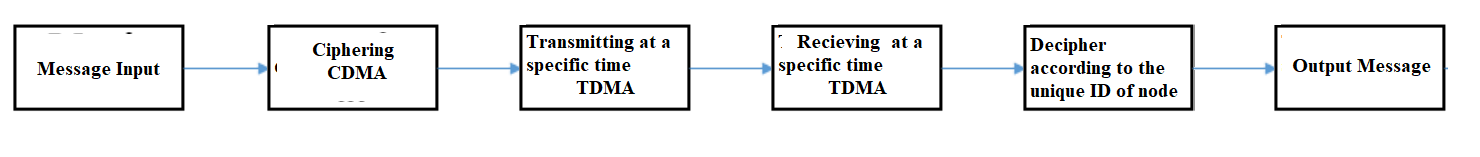
\includegraphics[scale = 0.59]{BlockDiagam.png}
 \caption{Block Diagram of the Solution presented}
 \end{figure}
 
 The input can be via a keypad/keyboard. The ciphering is done with respect to the ID of the intended reciever. The transmission is done at a specific time set aside for the intended reciever to recieve. The transmission is done via the RF transmitter module. The reciever than recieves in he selected slot. An optional task could be to implement an algorithm for multihop routing. After the intended reciever deciphers the message it can be displayed to the user via LEDs/screen output/LCD. 
 
 \section{Resource description}
 
 The following items will tentatively be required,
 
 \begin{itemize}
 \item Arduinos
 \item RF Modules
 \item MPU6050 (Gyroscopes)
 \item LCD Displays
 \item LEDs
 \item Connectors
 \end{itemize}


% --------------------------------------------------------------
%     You don't have to mess with anything below this line.
% --------------------------------------------------------------
 
\end{document}